\documentclass[letterpaper,12pt]{article}
\usepackage[english]{babel}
\usepackage{natbib}
\usepackage{url}
\usepackage[utf8x]{inputenc}
\usepackage{amsmath}
\usepackage{graphicx}
\graphicspath{{images/}}
\usepackage{parskip}
\usepackage{fancyhdr}
\usepackage{vmargin}
\usepackage{float}
\usepackage[hidelinks]{hyperref}
\usepackage{multirow}
\usepackage{listings}
\usepackage[pass]{geometry}
\usepackage[table,xcdraw]{xcolor}

% Set letter paper size:
\setlength{\paperheight}{11in}
\setlength{\paperwidth}{8.5in}




\usepackage{color}
\definecolor{codegreen}{rgb}{0,0.6,0}
\definecolor{codegray}{rgb}{0.5,0.5,0.5}
\definecolor{codepurple}{rgb}{0.58,0,0.82}
\definecolor{backcolour}{rgb}{0.95,0.95,0.92}

\setmarginsrb{3 cm}{2.5 cm}{3 cm}{2.5 cm}{1 cm}{1.5 cm}{1 cm}{1.5 cm}

\title{Watershed Delineation}								% Title
\author{Vahid Salahi}								% Author
\date{10 Feb 2017}											% Date

\makeatletter
\newcommand*{\rom}[1]{\expandafter\@slowromancap\romannumeral #1@}
\let\thetitle\@title
\let\theauthor\@author
\let\thedate\@date
\makeatother

\pagestyle{fancy}
\fancyhf{}
\rhead{\theauthor}
\lhead{\thetitle}
\cfoot{\thepage}

\begin{document}
	

%%%%%%%%%%%%%%%%%%%%%%%%%%%%%%%%%%%%%%%%%%%%%%%%%%%%%%%%%%%%%%%%%%%%%%%%%%%%%%%%%%%%%%%%%

\begin{titlepage}
	\centering
    \vspace*{0 cm}
    
\includegraphics[scale = 0.2]{logottu}\\[3.0 cm]	% University Logo
    \text{\LARGE Cypress Ck nr Westfield}\\[2.0 cm]
	\textsc{\Large }\\[0.1 cm]				% Course Code
	\rule{\linewidth}{0.1 mm} \\[0.4 cm]
	{ \huge \bfseries Spatial Hydrology}\\
	\rule{\linewidth}{0.2 mm} \\[1.5 cm]
	
	\begin{minipage}{0.4\textwidth}
		\begin{flushleft} \large
			\emph{Submitted By:}\\
			Vahid Salahi\\
			R11358400\\
            
		\end{flushleft}
	\end{minipage}~
	\begin{minipage}{0.4\textwidth}   
		\begin{flushright} \large
			\emph{Submitted To:} \\
			Dr.	Uddameri\\
		\end{flushright}
        
	\end{minipage}\\[2 cm]

~
    { March 15, 2017}\\[1 cm]
    
\end{titlepage}

%%%%%%%%%%%%%%%%%%%%%%%%%%%%%%%%%%%%%%%%%%%%%%%%%%%%%%%%%%%%%%%%%%%%%%%%%%%%%%%%%%%%%%%%%

\tableofcontents
\newpage
\listoffigures
\newpage
\listoftables
\pagebreak

%%%%%%%%%%%%%%%%%%%%%%%%%%%%%%%%%%%%%%%%%%%%%%%%%%%%%%%%%%%%%%%%%%%%%%%%%%%%%%%%%%%%%%%%%


\section*{Section 1}
\addcontentsline{toc}{section}{Section 2}
\textbf{Delineate the watershed for the USGS gaging station corresponding to USGS 08069000 Cypress Ck nr Westfield, TX.}
\\
\begin{enumerate}
	\item \textbf{Show the flow direction, flow accumulation, and the final watershed maps (not screenshots). At a minimum you map must contain a legend, a north arrow and a scale bar.}\\~
	
	The Digital Elevation Model has been used to derive flow direction map. The following prepossessing steps have been done to obtain the proper DEM to start the analysis:
\begin{itemize}
	\item Two DEM subcategories with $10\;m$ resolution ($1/3\;arc$) downloaded from \url{https://nationalmap.gov/} which cover the entire 8 digit HUC corresponding to station point.
	\item \emph{''UTM Zone 14 N''} was used as projection system to re-project both DEM subcategories. For this study, all the data and maps was projected using "UTM Zone 14N".
	\item \emph{"Mosaic to New Raster"} tool has been utilized to combine two DEMs to get one raster file.
	\item 8 digit HUC with number of 12040102 which is containing the station point, was used as \emph{"Clip"} feature to constrain the DEM raster data based on.
	\item \emph{"Fill"} tool was used to remove small imperfections.
\end{itemize}
		The final map of digital elevation model is depicted as Figure 1.
	\begin{figure}[H]
		\begin{center}
			\includegraphics[width=15cm]{DEMmap}
		\end{center}
		\caption{Digital Elevation Model Clipped to the corresponding 8 digit HUC}\label{DEM}
	\end{figure}
	
	
	Based on the corrected DEM, the flow direction and flow accumulation maps are generated, shown as Figure 2 and 3 respectively. The flow accumulation map looks very uniform with low accumulation for entire raster data because the number of cells with low accumulation is much higher than the number of cells with high accumulation. By zooming in, the streams of high accumulation cells can be seen. Figure 4 shows a closer view of the accumulation map corresponding to the vicinity area of the station point.
	
		\begin{figure}[H]
			\begin{center}
				\includegraphics[width=11cm]{flowdir2}
			\end{center}
			\caption{Flow direction map based on DEM}\label{flow_dir}
		\end{figure}

	\begin{figure}[H]
		\begin{center}
			\includegraphics[width=11cm]{flowacc2}
		\end{center}
	\caption{Flow accumulation map}\label{flow_acc_zoom}
	\end{figure}

	Figure 4 shows that the station point is not located on any cell with high accumulation (stream). The distance of $25\;m$ was measured from the station point to the near stream and used as the tolerance in \emph{"Snap Pour Point"} tool. The location of Pour Point on the stream is shown on Figure 4 in blue color.

	\begin{figure}[H]
		\begin{center}
			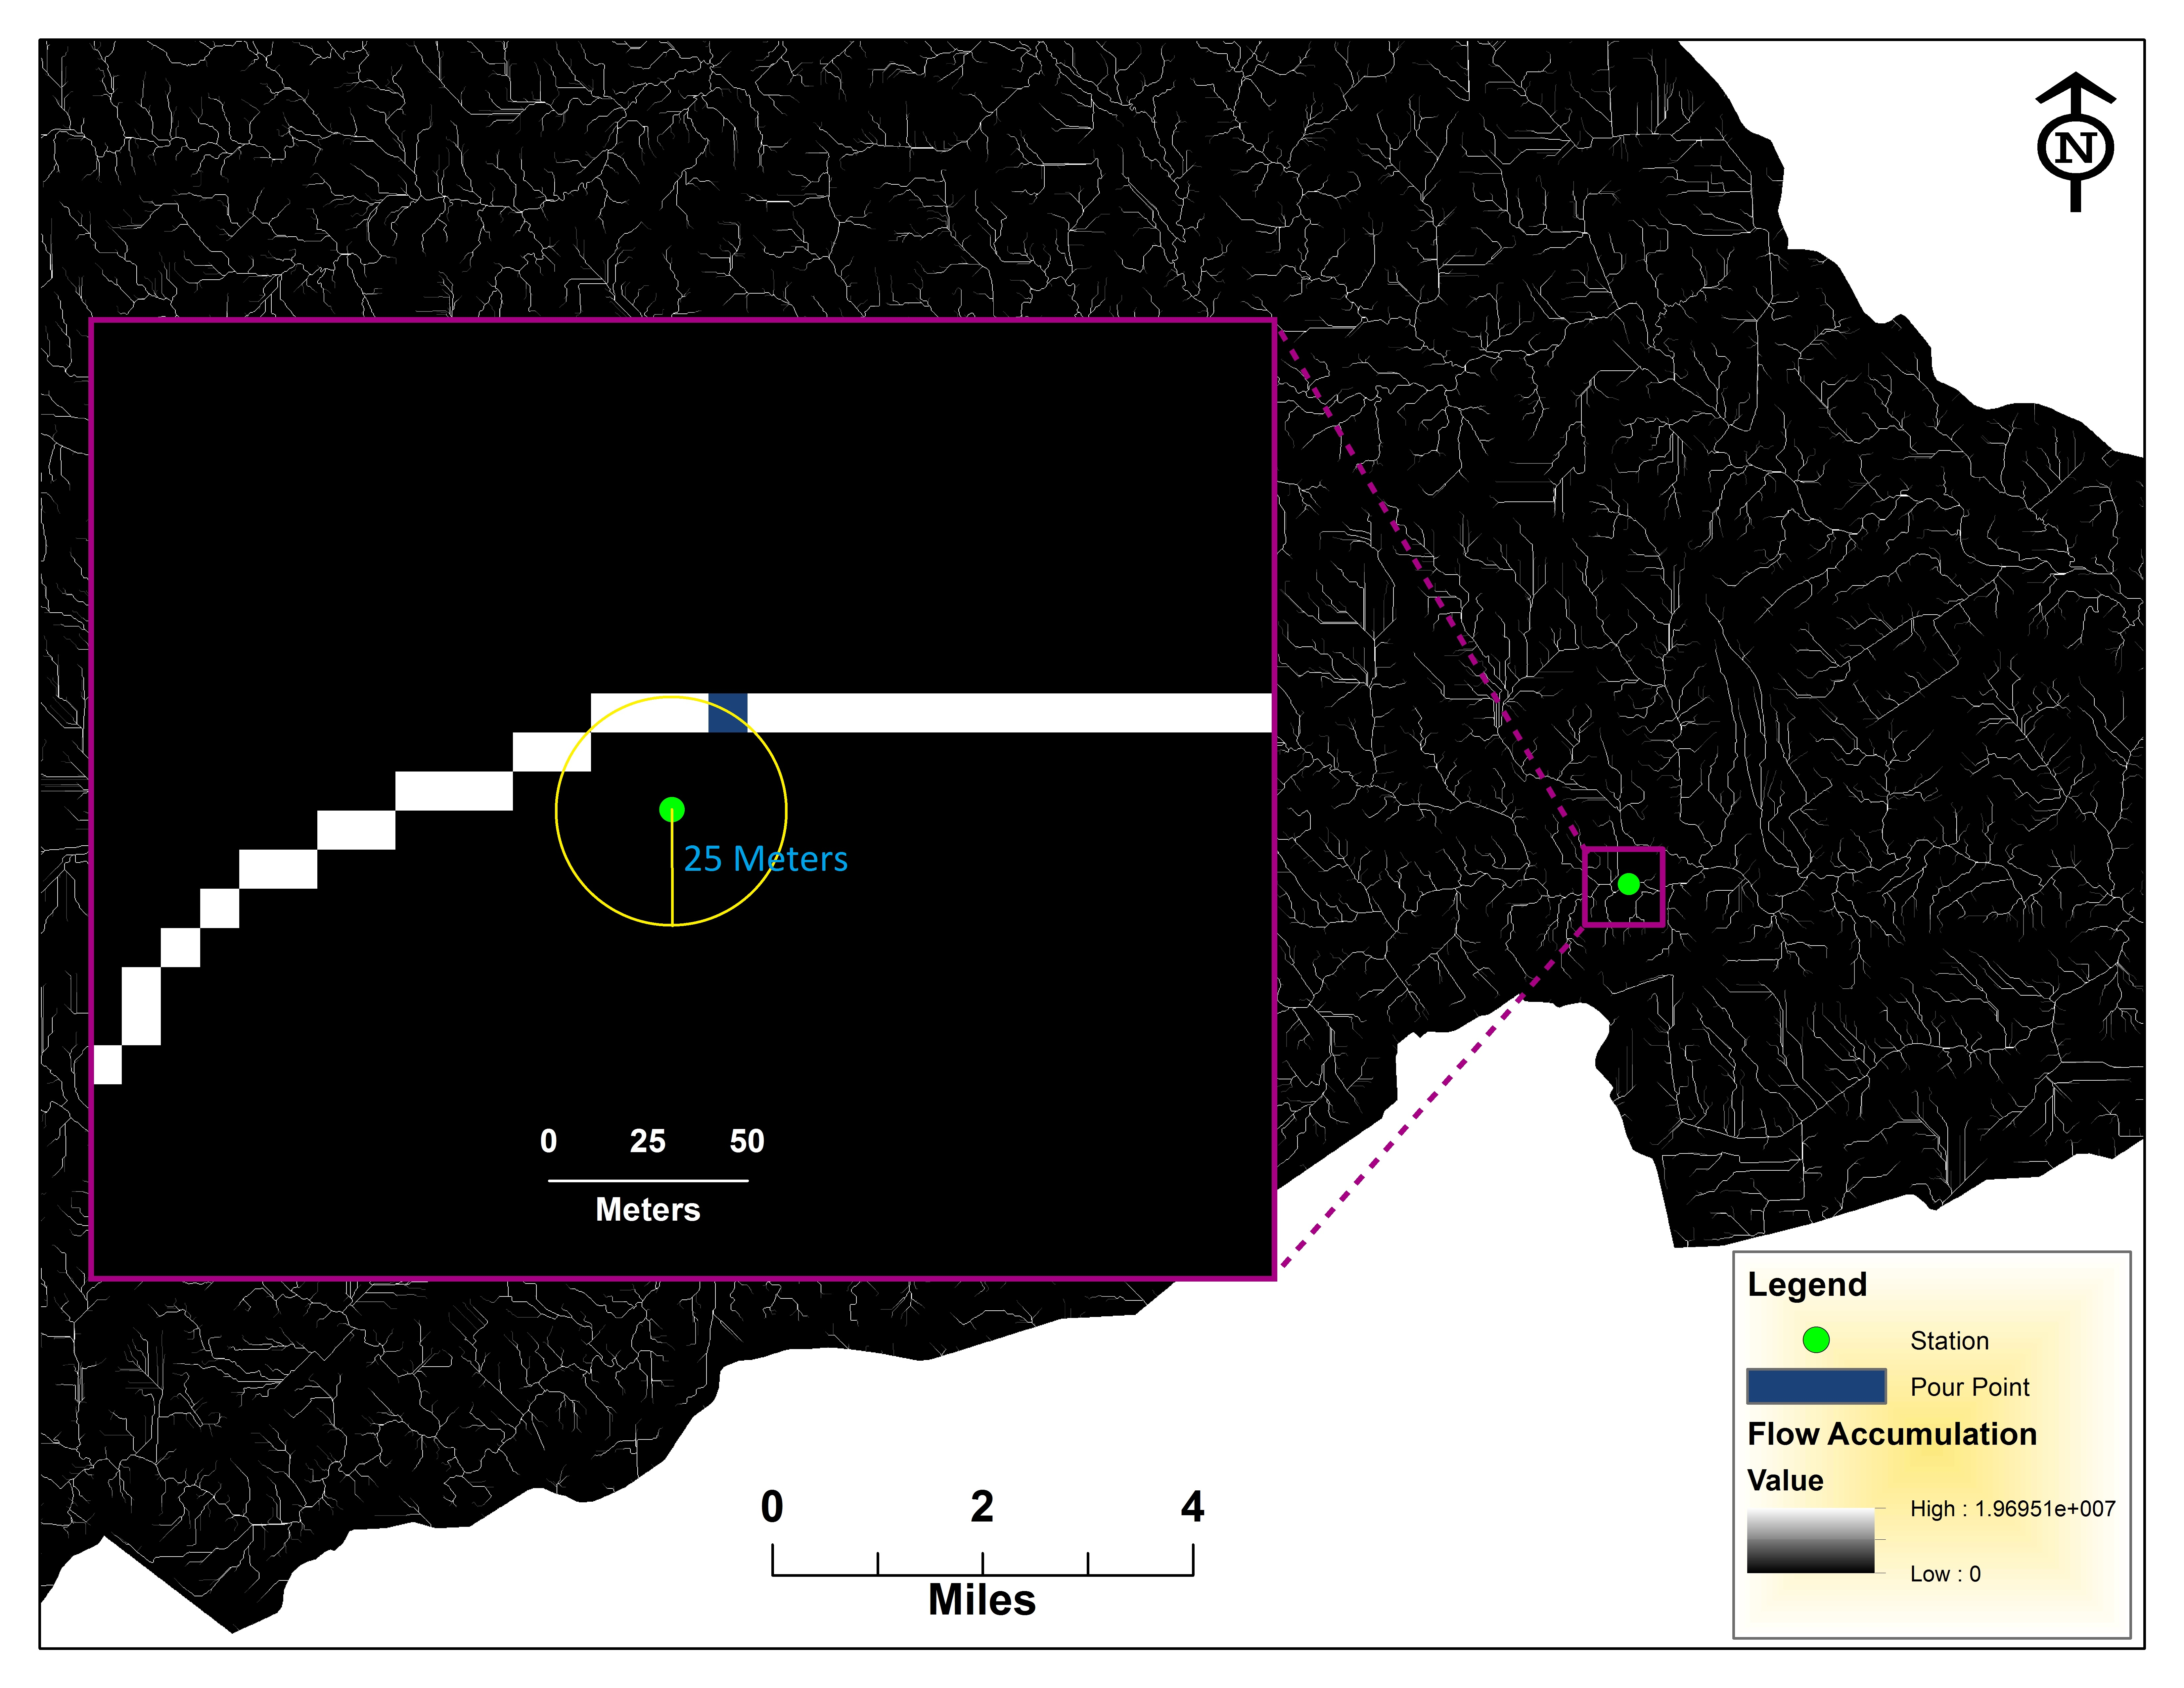
\includegraphics[width=16cm]{snappoint2}
		\end{center}
		\caption{Flow accumulation map (close view of the station point)}
	\end{figure}~


	\emph{"Watershed"} tool has been used to delineate the watershed associated with the snap pour point. The output watershed is shown in Figure 5.
	
	
	
	\begin{figure}[H]
		\begin{center}
			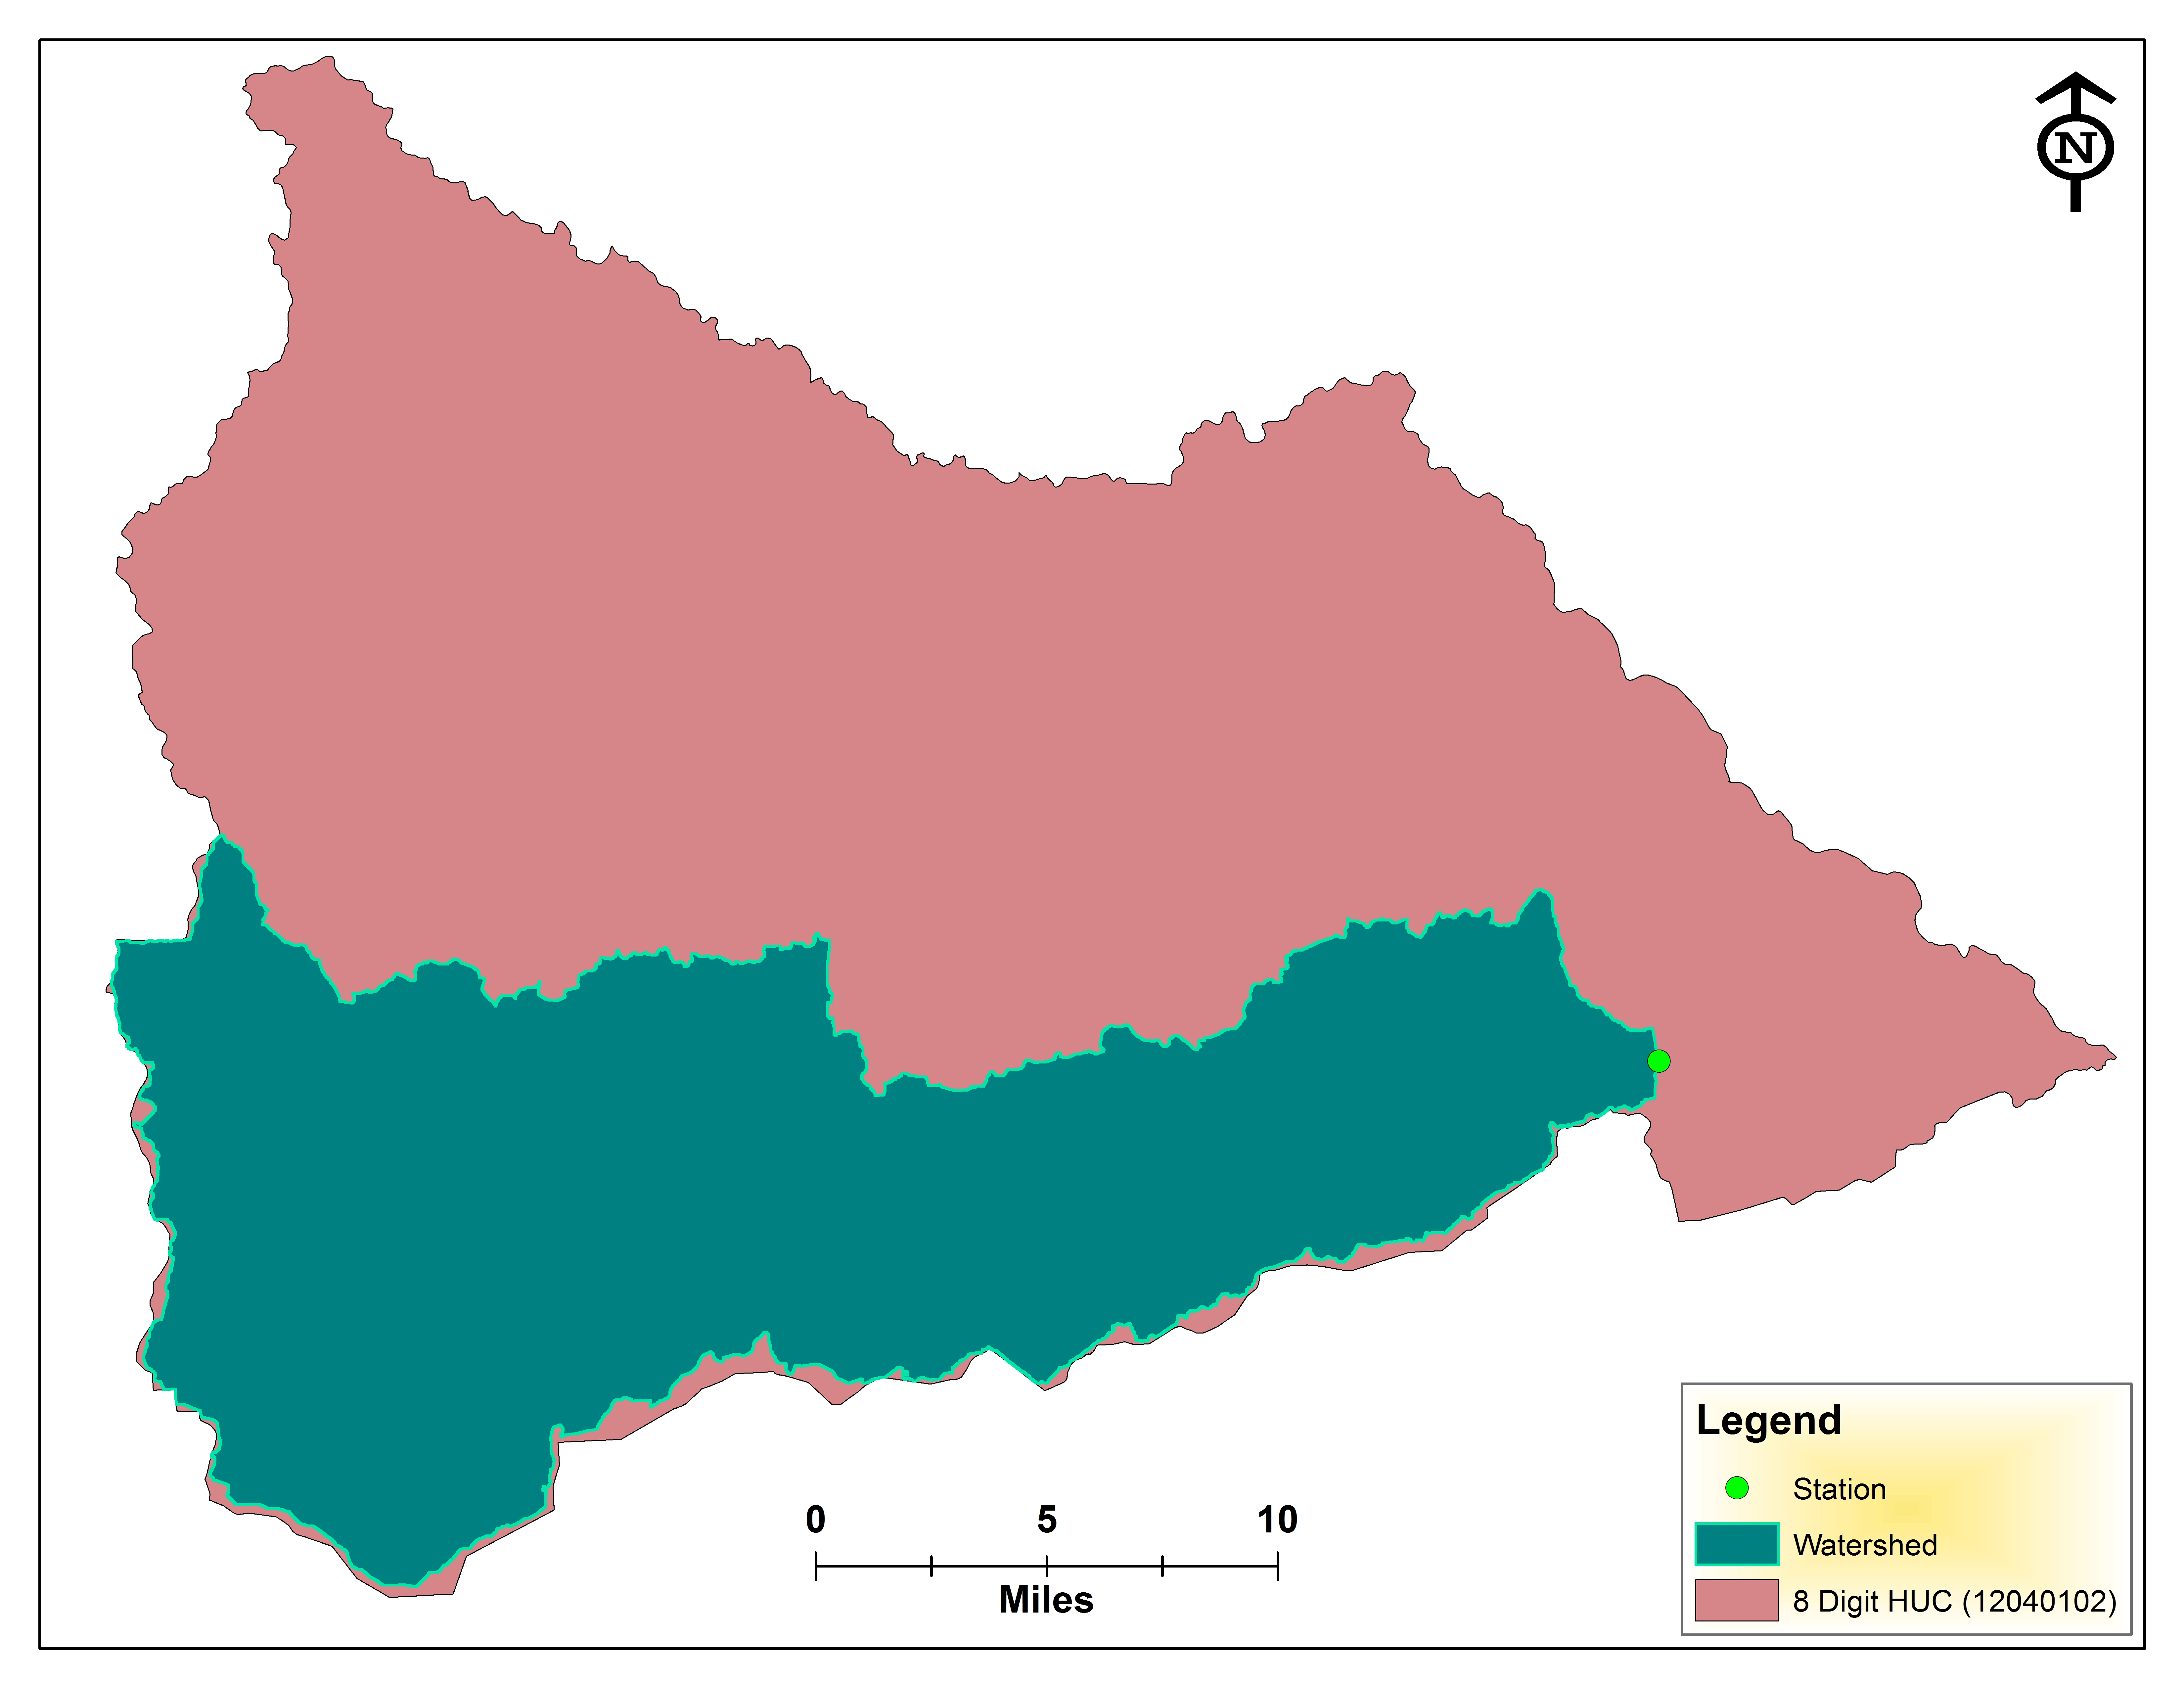
\includegraphics[width=16cm]{watershed2}
		\end{center}
		\caption{Watershed associated with pour point}\label{watshed_Station}
	\end{figure}

		
	~\item \textbf{Calculate the contributing drainage area. Does it match reasonably with that indicated by the USGS on their website.}\\~
	
	The area of delineated watershed shown in Figure 5 is calculated as $268\;mi^2$ (for obtaining the area, watershed was converted from raster to polygon using \emph{"Raster to Polygon"} tool and then the area of polygon has been calculated). USGS has indicated an area of $285\;mi^2$ for the corresponding watershed. Difference in area can be mainly due to pour point estimation. Here a $25\;m$ distance has been chosen as the tolerance but watershed is significantly sensitive to the pour point and different results might be obtained by changing the pour point. There are some other parameters that can affect the watershed delineation process such as the resolution of DEM and the projection used for analysis.\

	In the next part, a sensitivity analysis has been considered on the DEM resolution. A courser resolution of $30\;m$ ($1\;arc$) has been chosen for the same analysis and the results have been compared. Figure 6 shows the DEM prepared for analysis in $30\;m$ resolution.

	\begin{figure}[H]
		\begin{center}
			\includegraphics[width=16cm]{DEM(30m)}
		\end{center}
	\caption{Digital Elevation Map with $30m$ resolution}\label{dem30}
	\end{figure}~

	The new delineated watershed based on the new DEM (Figure 6) has been shown in Figure 7. The difference between two delineated watershed cannot be distinguished visually and they are similar to each other. The corresponding area for the new watershed calculated to be $267.5\;mi^2$, indicating almost no change in area (half square mile difference). Decreasing resolution from $10\;m$ to $30\;m$ did not affect the watershed delineation result significantly.\\
	The comparison of the delineated watersheds is summarized in Table 1. 	For the rest of analysis, the delineated watershed from $10 \; m$ resolution DEM has been taken to consideration.
	
	
	
	\begin{figure}[H]
		\begin{center}
			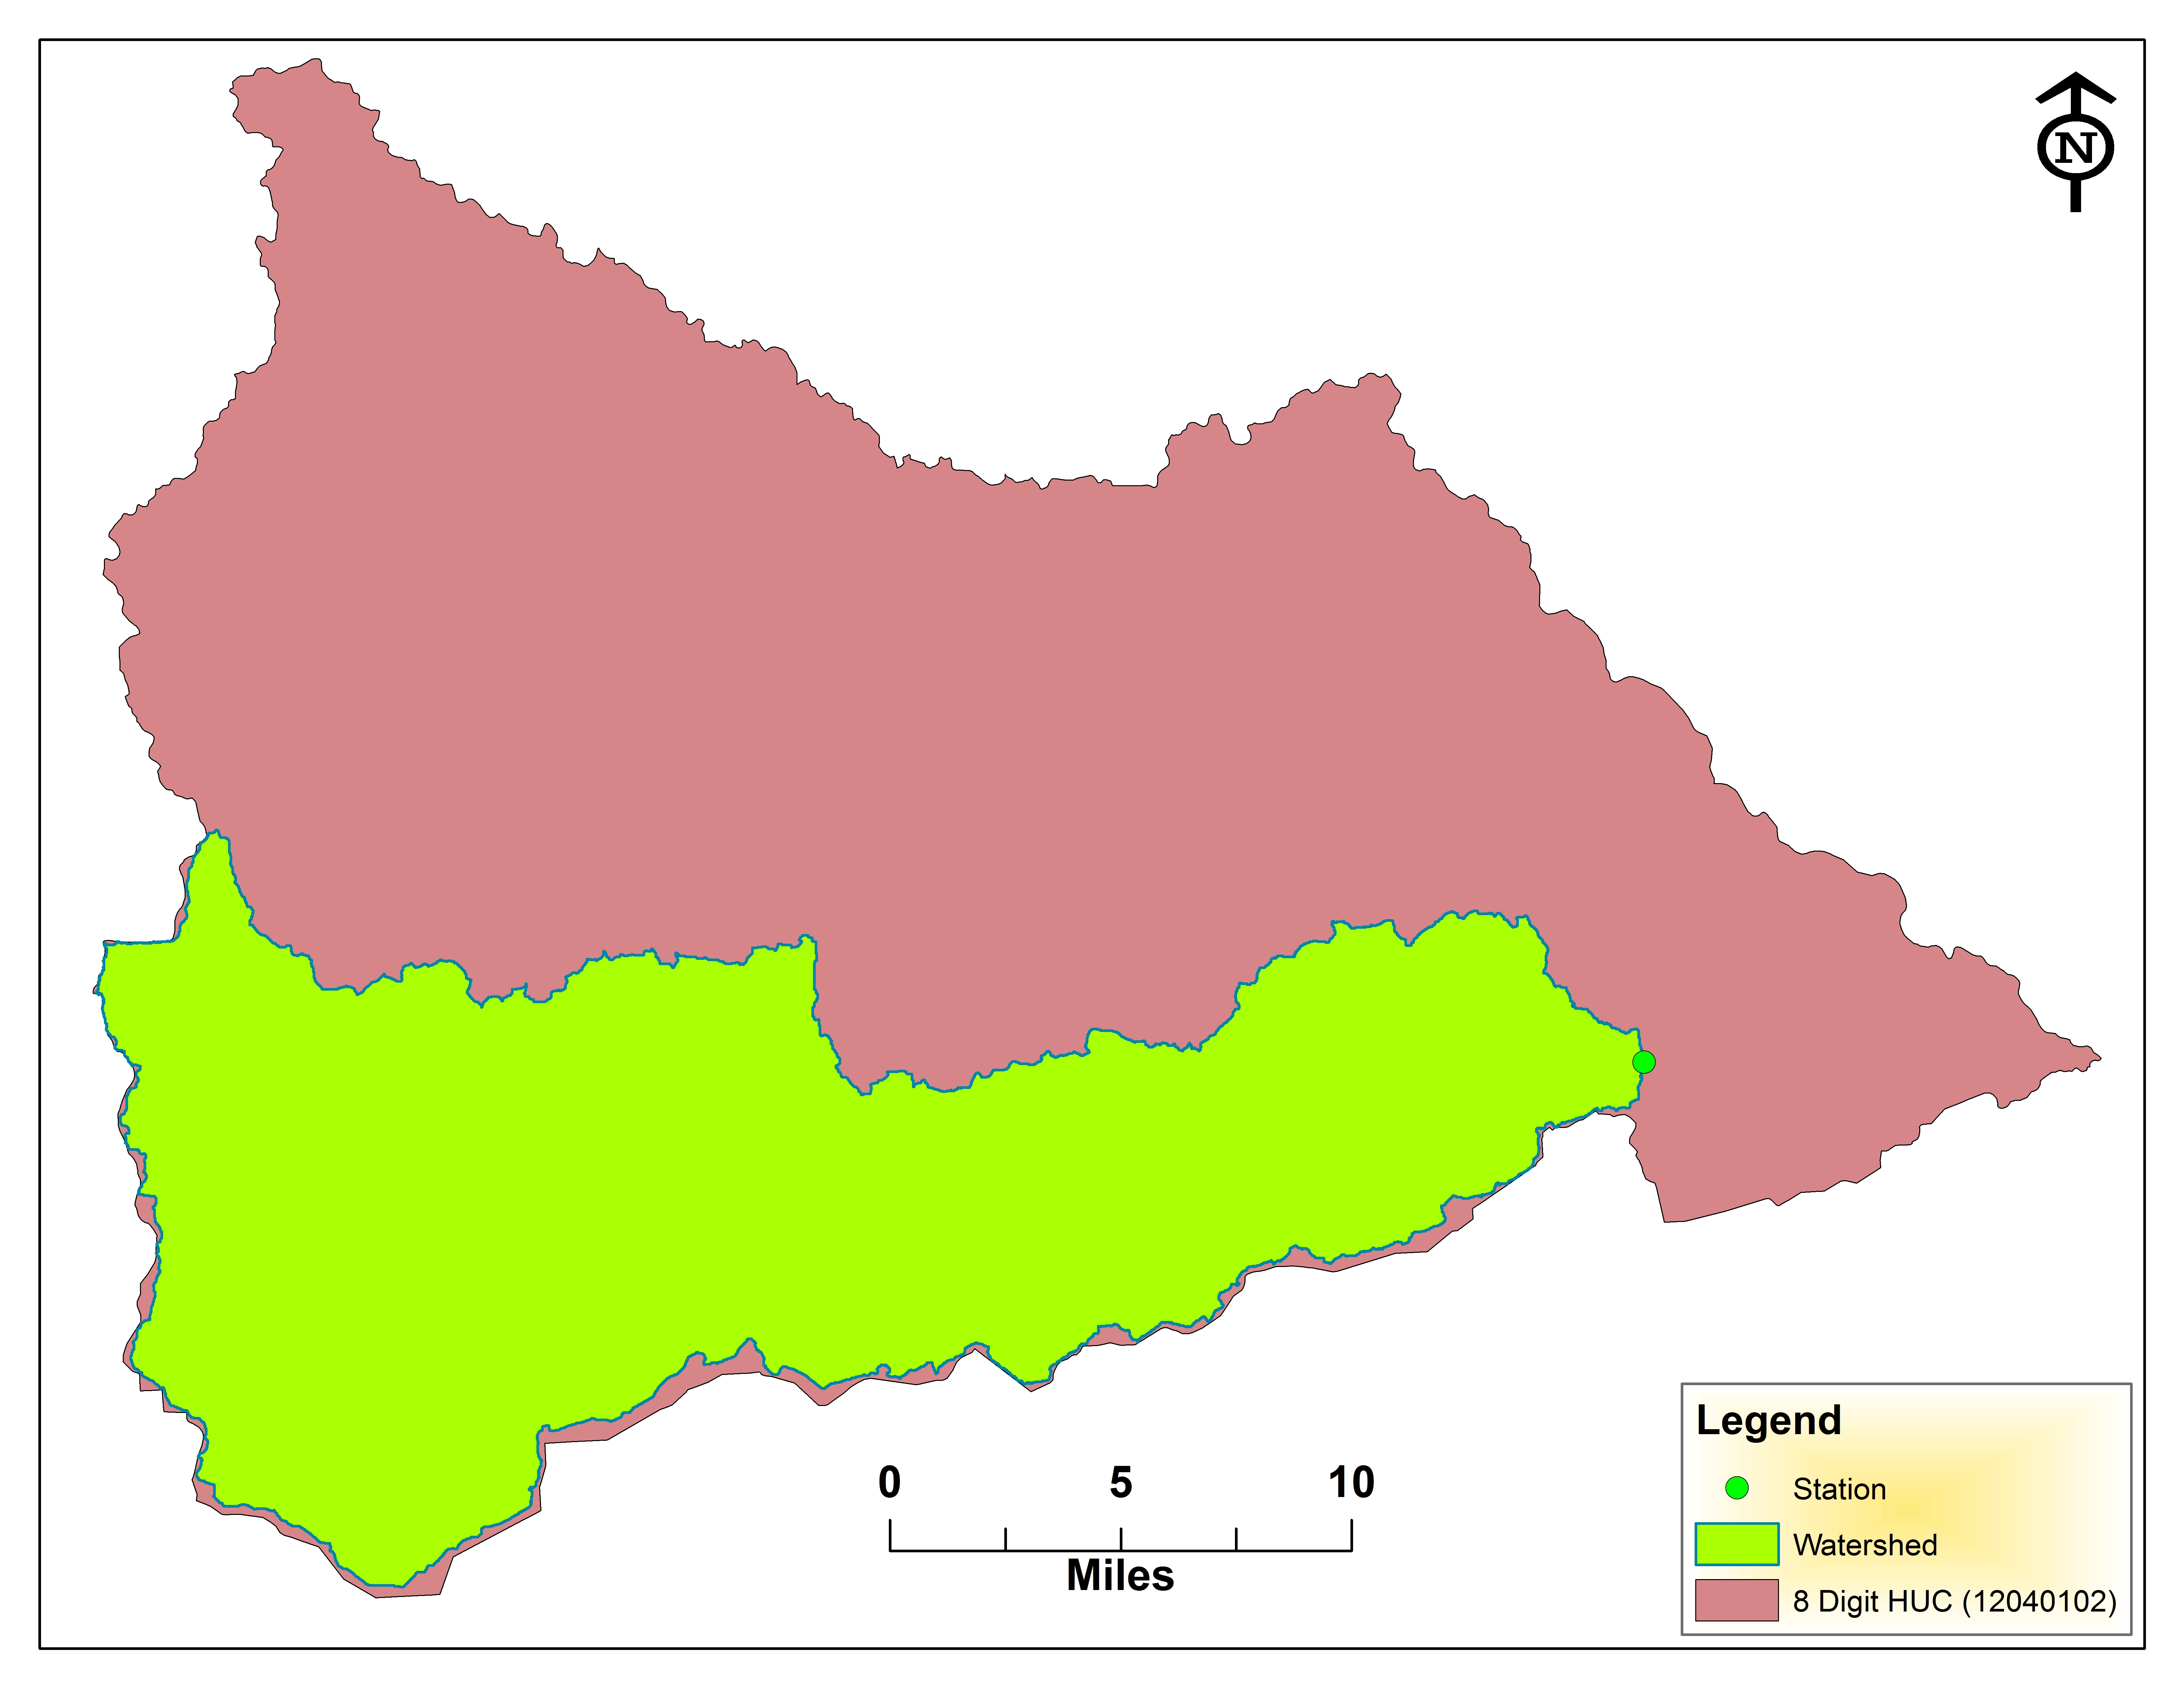
\includegraphics[width=16cm]{watershed(30m)2}
		\end{center}
	\caption{Watershed ($30m$ resolution)}\label{wsh30}
	\end{figure}

	\begin{table}[H]
	\centering
	\caption{Comparison of Watershed Areas}
	\label{my-label}
	\begin{tabular}{|l|c|c|}
		\hline
		Description & \multicolumn{1}{l|}{Area $mi^2$} & \multicolumn{1}{l|}{\% Difference to USGS Watershed} \\ \hline
		Watershed from USGS Website & 285 &  \\ \hline
		Watershed using DEM of 1/3 arc resolution & 268 & 5.96 \% \\ \hline
		Watershed using DEM of 1 arc resolution & 267.5 & 6.14 \% \\ \hline
		\end{tabular}
	\end{table}
	



\end{enumerate}

\newpage
\section*{Section 2}
\addcontentsline{toc}{section}{Section 3}
\textbf{Download or extract the following data pertinent to the watershed – Soil Hydrologic Group (SHG) using SSURGO and Soil Hydrologic Group (SHG) corresponding to STATSGO2}
\\
\begin{enumerate}
	\item \textbf{Develop SHG maps corresponding to these two datasets.}\\~
	
	The SHG map for both cases of SSURGO and STATSGO2 are shown in Figure 8 and Figure 9 respectively. For SSURGO case, the SHG for two counties of Harris and Waller have been \emph{clipped} to the watershed and then \emph{merged} to create the complete coverage of SHG on watershed. To obtain SHG using STATSGO2, the data of Texas state has been clipped to the watershed.

	\begin{figure}[H]
		\begin{center}
			\includegraphics[width=14cm]{SHG(SSURGO)}
		\end{center}
	\caption{SHG map of watershed using SSURGO}
	\end{figure}

	\begin{figure}[H]
		\begin{center}
			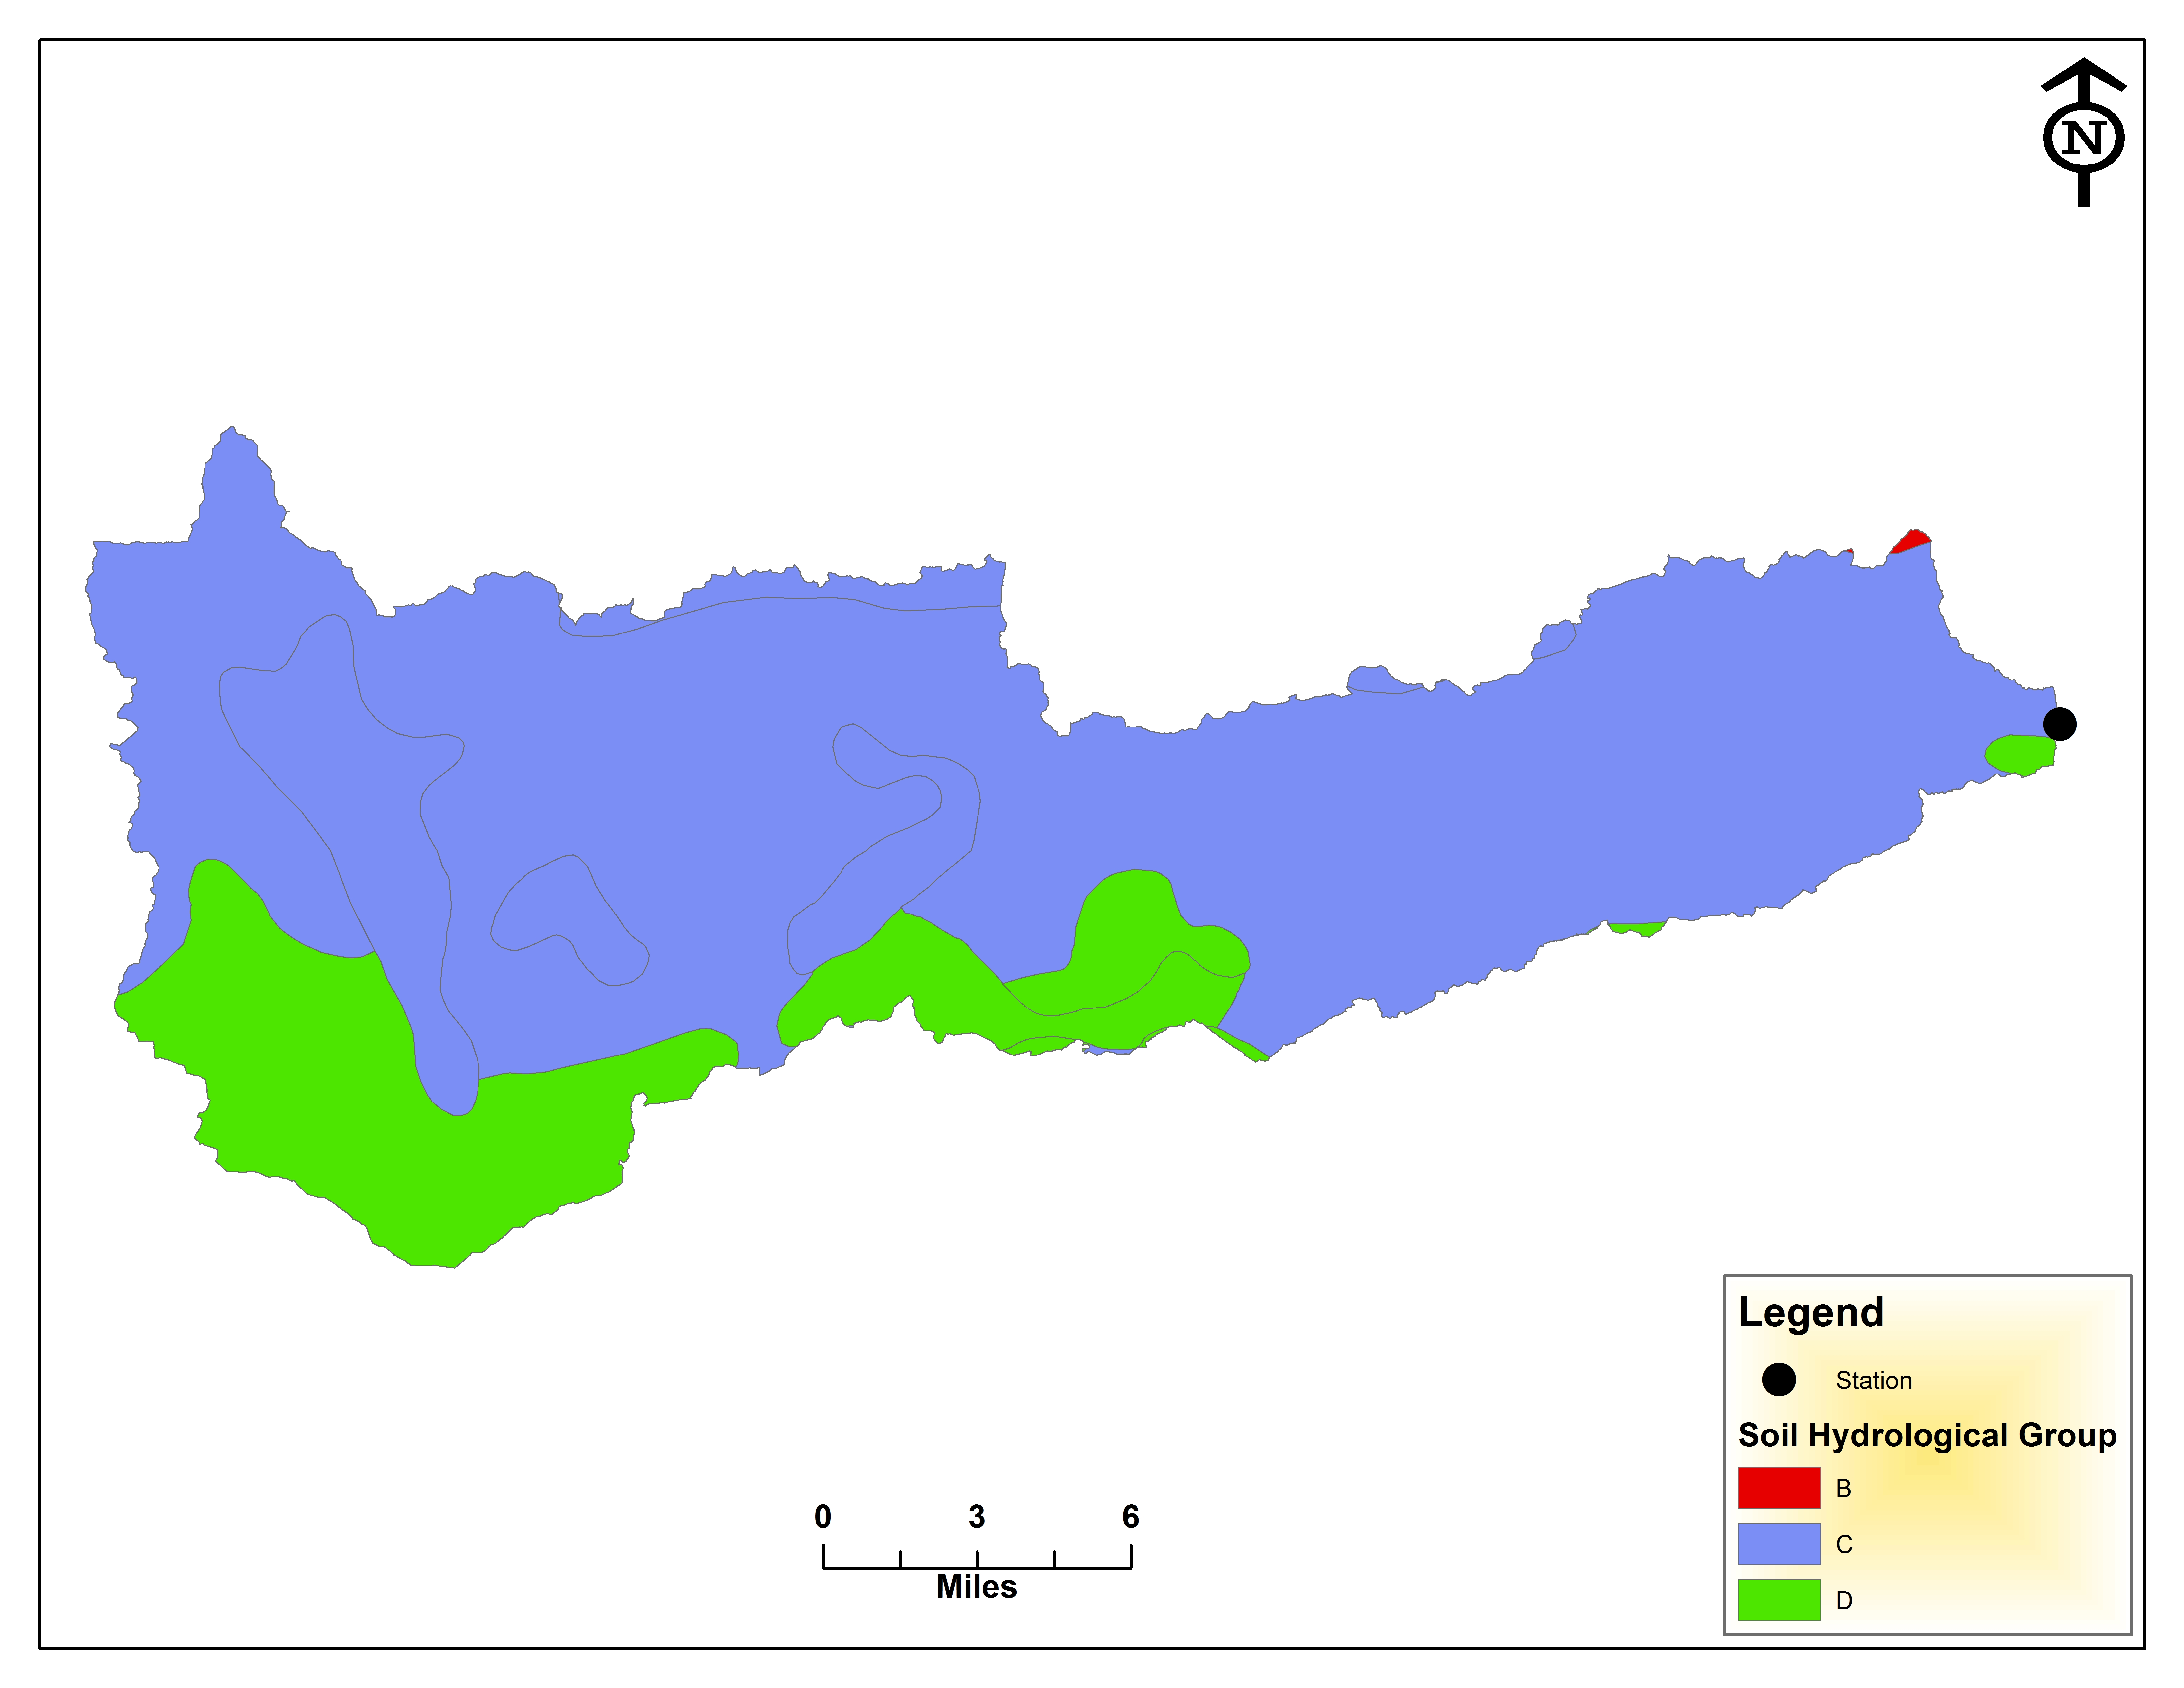
\includegraphics[width=16cm]{SHG(STATSGO2)}
		\end{center}
		\caption{SHG map of watershed using STATSGO2}
	\end{figure}~

	~\item \textbf{Discuss the difference between the two delineations.}\\~
	
	As it can be seen from Figure 8 and 9, these two delineations are different. The SHG map developed from STATGO2 has lost many details of SHG data and only have three class of SHG. But, the SHG map developed by SSURGO has more details of SHG distribution on the watershed. The other difference that can be observed is the lack of consistency between to delineations. For instance, the southern west part of the watershed has different SHG of C and D in these two delineation. Also, we can see significant areas of watershed in west are grouped as B in SSURGO, however, in STATGO2 delineation, there is very small area of group B which is located in the northern east. This failure in correspondence is another difference in these two methods of delineation.
	The SHG map from SSURGO delineation has been chosen for the rest of analysis.
	Table 2 has summarized the percentage area of each SHG corresponding to Both SSURGO and STATGO2. For SSURGO, B/D and C/D have been considered as B and C respectively. This reclassification has been taken with the assumption of pre-development analysis.
	
	\begin{table}[H]
		\centering
		\caption{Soil Hydrological Groups of Watershed}
		\label{my-label}
		\begin{tabular}{|c|c|c|}
			\hline
			Soil Hydrological Group & \multicolumn{1}{l|}{\% Area (SSURGO)} & \multicolumn{1}{l|}{\% Area (STATGO2)} \\ \hline
			A & 1.3 & 0 \\ \hline
			B & 17 & 0.1 \\ \hline
			C & 65.1 & 81.3 \\ \hline
			D & 16.6 & 18.7 \\ \hline
		\end{tabular}
	\end{table}
	
	
	
\end{enumerate}

\newpage

\section*{Section 3}	
\addcontentsline{toc}{section}{Section 4}
\textbf{Download the Land Use Land Cover (LULC) maps for the watershed for the years 2006 and 2011.}
\\
\begin{enumerate}
	\item \textbf{Map the LULC for these two years.}\\~
	
	The LULC map for entire US was obtained from USDA web soil survey. Figure 10 and 11 represent the LULC maps clipped to the delineated watershed for year 2006 and 2011 respectively. All the maps are projected to UTM zone 14N as well.
	
	\begin{figure}[H]
		\begin{center}
			\includegraphics[width=16cm]{lulc2006_2.jpg}
		\end{center}
		\caption{LULC map for the year 2006}
	\end{figure}~
	
	\begin{figure}[H]
		\begin{center}
			\includegraphics[width=16cm]{lulc2011_2.jpg}
		\end{center}
		\caption{LULC map for the year 2011}
	\end{figure}~
	
	~\item \textbf{Make a separate map that shows the areas that have undergone land use changes within that 5 year period.}\\~
	
	Figure 12 depicts all the places that LULC record has been changed from 2006 to 2011. This map has been obtained by comparison of LULC data corresponding two years of 2006 and 2011. \emph{"Raster Calculator"} was used to obtain the places that LULC has been changed.

	\begin{figure}[H]
		\begin{center}
			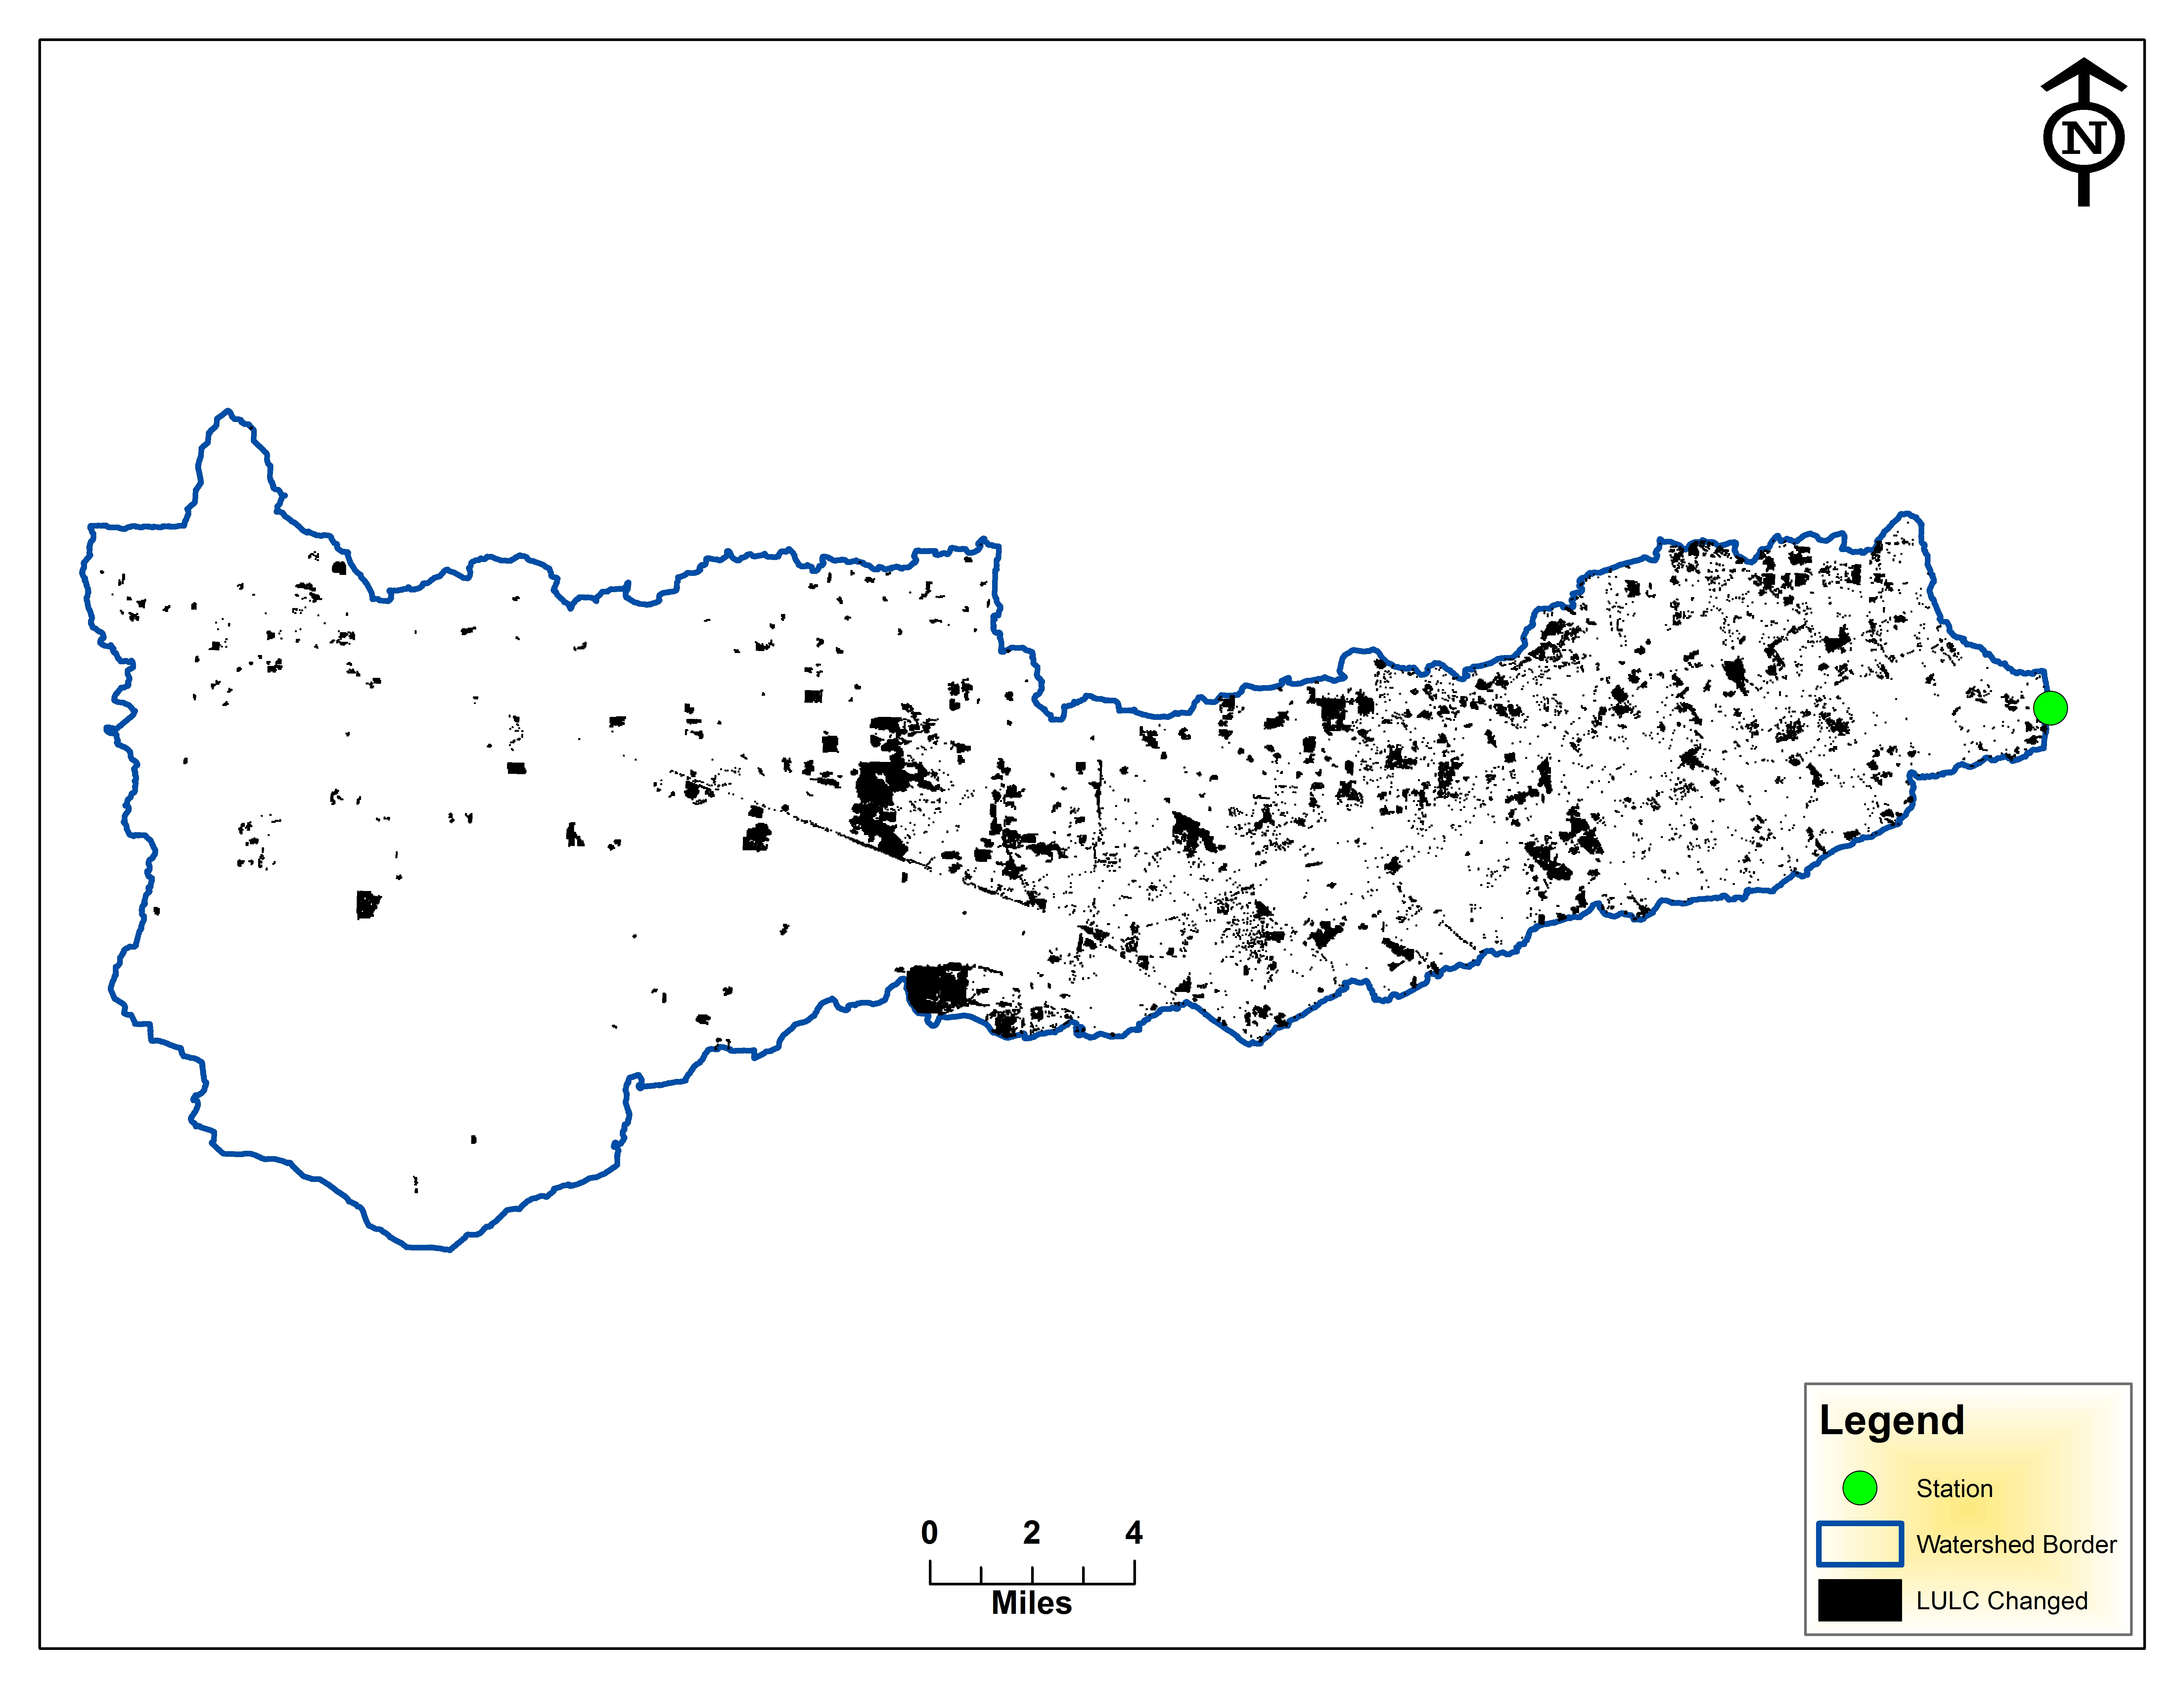
\includegraphics[width=16cm]{LULCchangel_2}
		\end{center}
		\caption{Landuse changes from 2006 to 2011}
	\end{figure}~
	
		~\item \textbf{How has the land use changed in the watershed within the 5 year period? Which LULC has the most dominant change?}\\~
	
	The total area of the watershed that has undergone land use changes is $12.89\;mi^2$. This value was obtained by converting the raster data shown in Figure 12 to polygon and then calculating the area. Table 3 shows the change of LULC from year 2006 to 2011 for all individual LULC classes.\\


\begin{table}[]
	\centering
	\caption{Change in Land Use Land Cover from 2006 to 2011}
	\label{my-label}
	\begin{tabular}{|l|c|c|c|}
		\hline
		Class Code and Name               & \multicolumn{1}{l|}{Area in 2006 (\%)} & \multicolumn{1}{l|}{Area in 2011 (\%)} & \multicolumn{1}{l|}{Change (\%)} \\ \hline
		11 (Open Water)                   & 0.51                                   & 0.72                                   & 0.21                             \\ \hline
		21 (Developed, Open Space)        & 11.12                                  & 10.74                                  & -0.38                            \\ \hline
		22 (Developed, Low Intensity)     & 9.99                                   & 10.73                                  & 0.74                             \\ \hline
		23 (Developed, Medium Intensity)  & 9.23                                   & 10.78                                  & 1.55                             \\ \hline
		24 (Developed High Intensity)     & 1.65                                   & 2.26                                   & 0.61                             \\ \hline
		31 (Barren Land)                  & 0.92                                   & 0.89                                   & -0.03                            \\ \hline
		41 (Deciduous Forest)             & 2.07                                   & 1.84                                   & -0.23                            \\ \hline
		42 (Evergreen Forest)             & 3.39                                   & 2.8                                    & -0.59                            \\ \hline
		43 (Mixed Forest)                 & 0.6                                    & 0.53                                   & -0.07                            \\ \hline
		52 (Shrub/Scrub)                  & 1.96                                   & 2                                      & 0.03                             \\ \hline
		71 (Grassland/Herbaceous)         & 1.8                                    & 1.91                                   & 0.11                             \\ \hline
		81 (Pasture/Hay)                  & 37.9                                   & 36.44                                  & -1.46                            \\ \hline
		82 (Cultivated Crops)             & 12.46                                  & 12.22                                  & -0.24                            \\ \hline
		90 (Woody Wetlands)               & 5.07                                   & 4.83                                   & -0.24                            \\ \hline
		95 (Emergent Herbaceous Wetlands) & 1.32                                   & 1.32                                   & 0                                \\ \hline
	\end{tabular}
\end{table}

The class code presented in Table 3 are encoded according to the USGS land cover institute (LCI). Based on this table, the highest change of LULC in the watershed is in Residential (Medium Intensity). $1.55\;\%$ of watershed area has been increased for LULC class of 23. Also, land use corresponding to class 81 which is indicating Pasture/Hay land use has been decreased by $1.46\;\%$. These changes imply lower capacity of infiltration and higher capacity of runoff for the watershed. 

\end{enumerate}



\newpage
\section*{Section 4}
\addcontentsline{toc}{section}{Section 5}
\textbf{Use the 2011 LULC and SSURGO SHG datasets to develop a spatial distribution of the Curve Number within the watershed.}
\\
\begin{enumerate}
	\item \textbf{Show a map of the spatial distribution of the Curve Number within the watershed.}\\~
	
	The 2011 LULC includes 15 classes of different land uses. Table 4 shows the reclassification of LULC in four major classes. This reclassifications has been done to make the task easier. 

\begin{table}[H]
	\centering
	\caption{Reclassification of LULC data}
	\label{lulcreclass}
	\begin{tabular}{|c|l|c|c|}
		\hline
		\multicolumn{2}{|c|}{\textbf{Original LULC Classification}} & \multicolumn{2}{c|}{\textbf{Reclassification}}                 \\ \hline
		Class Number&Description&New Class Num&Description                  \\ \hline
		11&Opern Water& \multirow{3}{*}{1} & \multirow{3}{*}{Water} \\ \cline{1-2}
		90&Woody Wetlands&&\\ \cline{1-2}
		95&Emergent Herbaceous Wetlands&& \\ \hline
		21&Developed, Open Space& \multirow{4}{*}{2} & \multirow{4}{*}{Residential} \\ \cline{1-2}
		22&Developed, Low Intensity&&\\ \cline{1-2}
		23&Developed, Medium Intensity&&\\ \cline{1-2}
		24&Developed High Intensity&&\\ \hline
		41&Deciduous Forest& \multirow{3}{*}{3} & \multirow{3}{*}{Forest} \\ \cline{1-2}
		42&Evergreen Forest&&\\ \cline{1-2}
		43&Mixed Forest&&\\ \hline
		31&Barren Land& \multirow{5}{*}{4} & \multirow{5}{*}{Agriculture} \\ \cline{1-2}
		52&Shrub/Scrub&&\\ \cline{1-2}
		71&Grassland/Herbaceous&&\\ \cline{1-2}
		81&Pasture/Hay&&\\ \cline{1-2}
		82&Cultivated Crops&&\\ \hline
	\end{tabular}
\end{table}
	
	Figure 13 shows the spatial distribution of reclassified LULC on the watershed. The reclassification has been done using \emph{"Reclassify"} toll in ArcGIS and 2011 LULC rater data was used as input.
		
	\begin{figure}[H]
		\begin{center}
			\includegraphics[width=16cm]{lulc2011reclass_2}
		\end{center}
		\caption{Reclassified LULC of 2011}\label{lulcmod}
	\end{figure}~

	Based on Figure 8, there are some regions that SHG are assigned as B/D or C/D. Assuming pre-development evaluation of the watershed, SHG of B and C was substituted for groups B/D and C/D respectively. The spatial distribution of the new SHG dataset is shown in Figure 14.  
	
	\begin{figure}[H]
		\begin{center}
			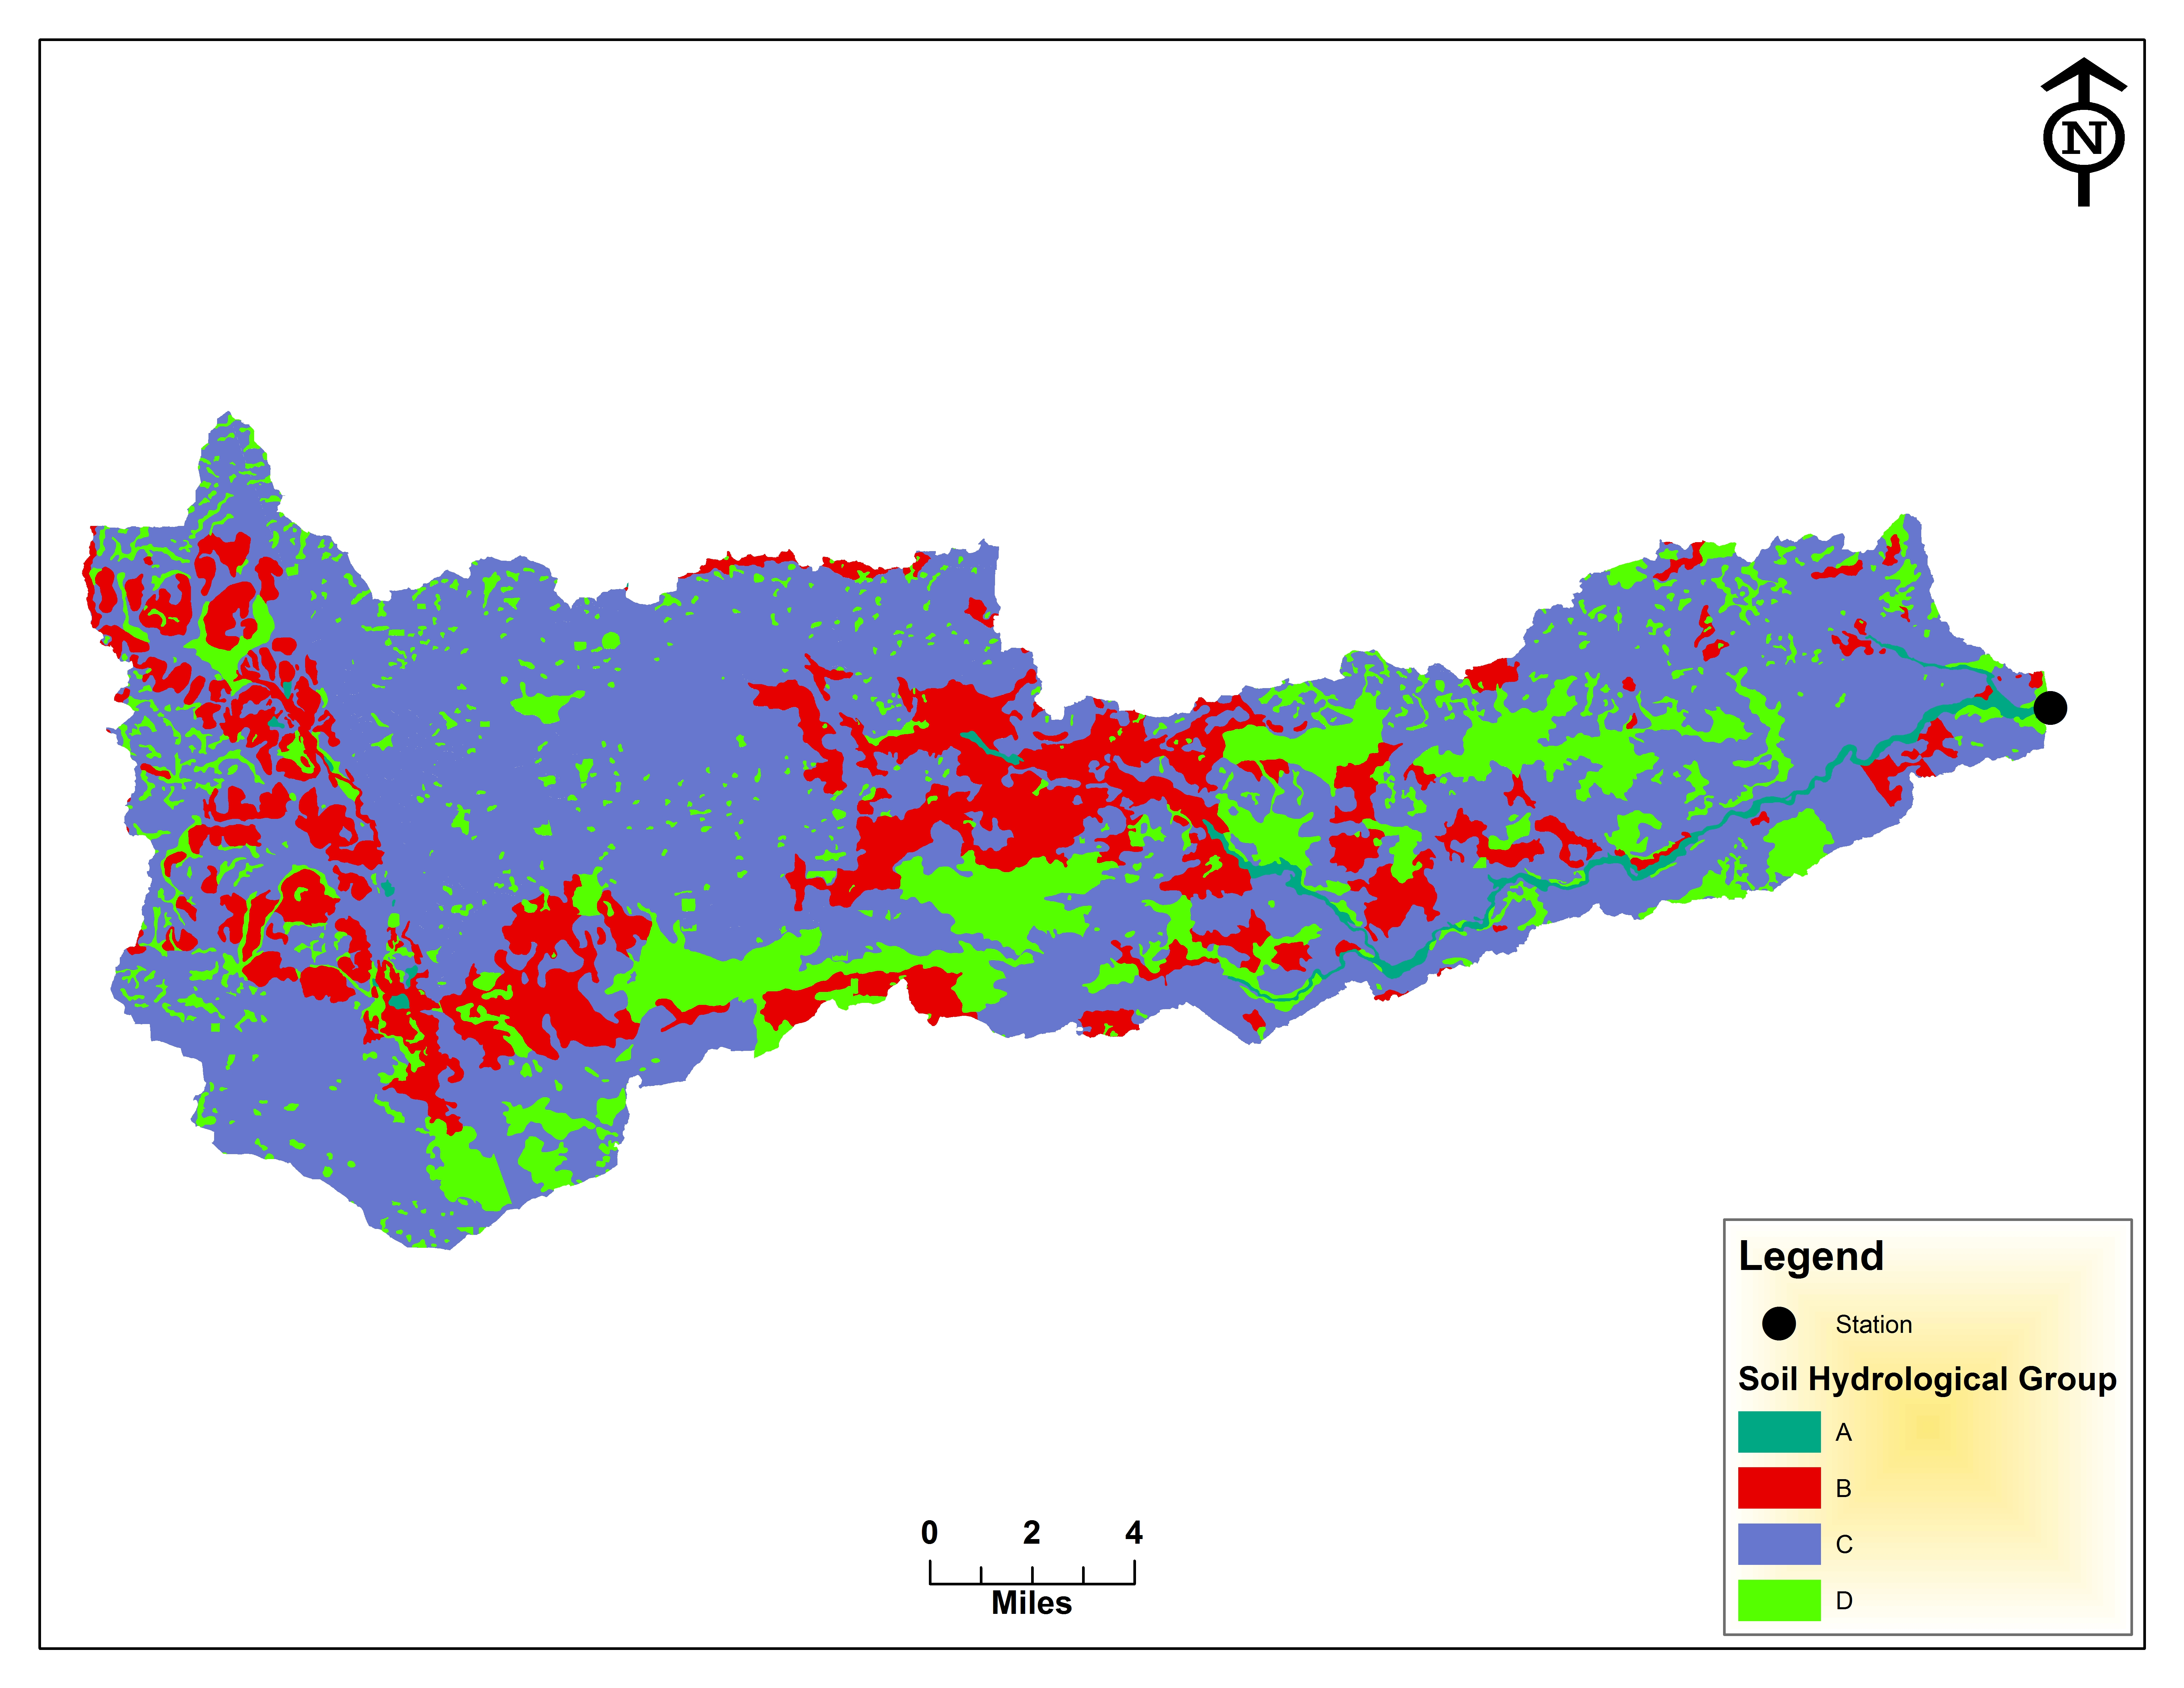
\includegraphics[width=16cm]{SHG(modif)_2}
		\end{center}
		\caption{Reclassified SHG using SSURGO delineation}\label{SHGmod}
	\end{figure}~
	
	After preparation of LULC and SHG data, a fishnet of $50\times 50\;m$ cell size was created covering the watershed. \emph{"Spatial Join"} tool was used to spatially join LULC and SHG data to each cell of fishnet. The LULC and SHG are going to be used in conjunction with curve numbers, to assign a curve number to each cell of fishnet. Table 5 summarize the curve numbers associated with pairs of LULCs and SHGs. Classification of Table 4 and 5 were done by using datasets presented in our text book and also a report with topic of \emph{"Creating SCS Curve Number Grid using HEC-GeoHMS"} which was prepared by Venkatesh Merwade from Purdue University. This report is available online (\url{https://web.ics.purdue.edu/~vmerwade/education/cngrid.pdf}).
	
\begin{table}[H]
	\centering
	\caption{Curve Number}
	\begin{tabular}{|l|c|c|c|c|}
		\hline
		\multicolumn{1}{|c|}{\multirow{2}{*}{LULC}} & \multicolumn{4}{c|}{Soil Hydrological Gropup} \\ \cline{2-5} 
		\multicolumn{1}{|c|}{}                      & A         & B         & C         & D         \\ \hline
		1 (Water)                                   & 100       & 100       & 100       & 100       \\ \hline
		2 (Residential)                             & 77        & 81        & 86        & 91        \\ \hline
		3 (Forest)                                  & 30        & 58        & 71        & 78        \\ \hline
		4 (Agriculture)                             & 67        & 77        & 83        & 87        \\ \hline
	\end{tabular}
\end{table}

\lstdefinestyle{mystyle}{
	backgroundcolor=\color{backcolour},   
	commentstyle=\color{codegreen},
	keywordstyle=\color{blue},
	numberstyle=\tiny\color{codegray},
	stringstyle=\color{codepurple},
	basicstyle=\footnotesize,
	breakatwhitespace=false,         
	breaklines=true,                 
	captionpos=b,                    
	keepspaces=true,                 
	numbers=left,                    
	numbersep=5pt,                  
	showspaces=false,                
	showstringspaces=false,
	showtabs=false,                  
	tabsize=2
}

\lstset{style=mystyle}


	The following code has been written in R to assign the curve numbers to the fishnet cells based of Table 5.\\
	
	\lstinputlisting[language=R]{CNcode.R}~

	The processed fishnet dataset was taken back to ArcGIS including the new attribute of Curve Number (CN). Figure 15 shows the spatial distribution of curve number on the watershed.\\
	
	\begin{figure}[H]
		\begin{center}
			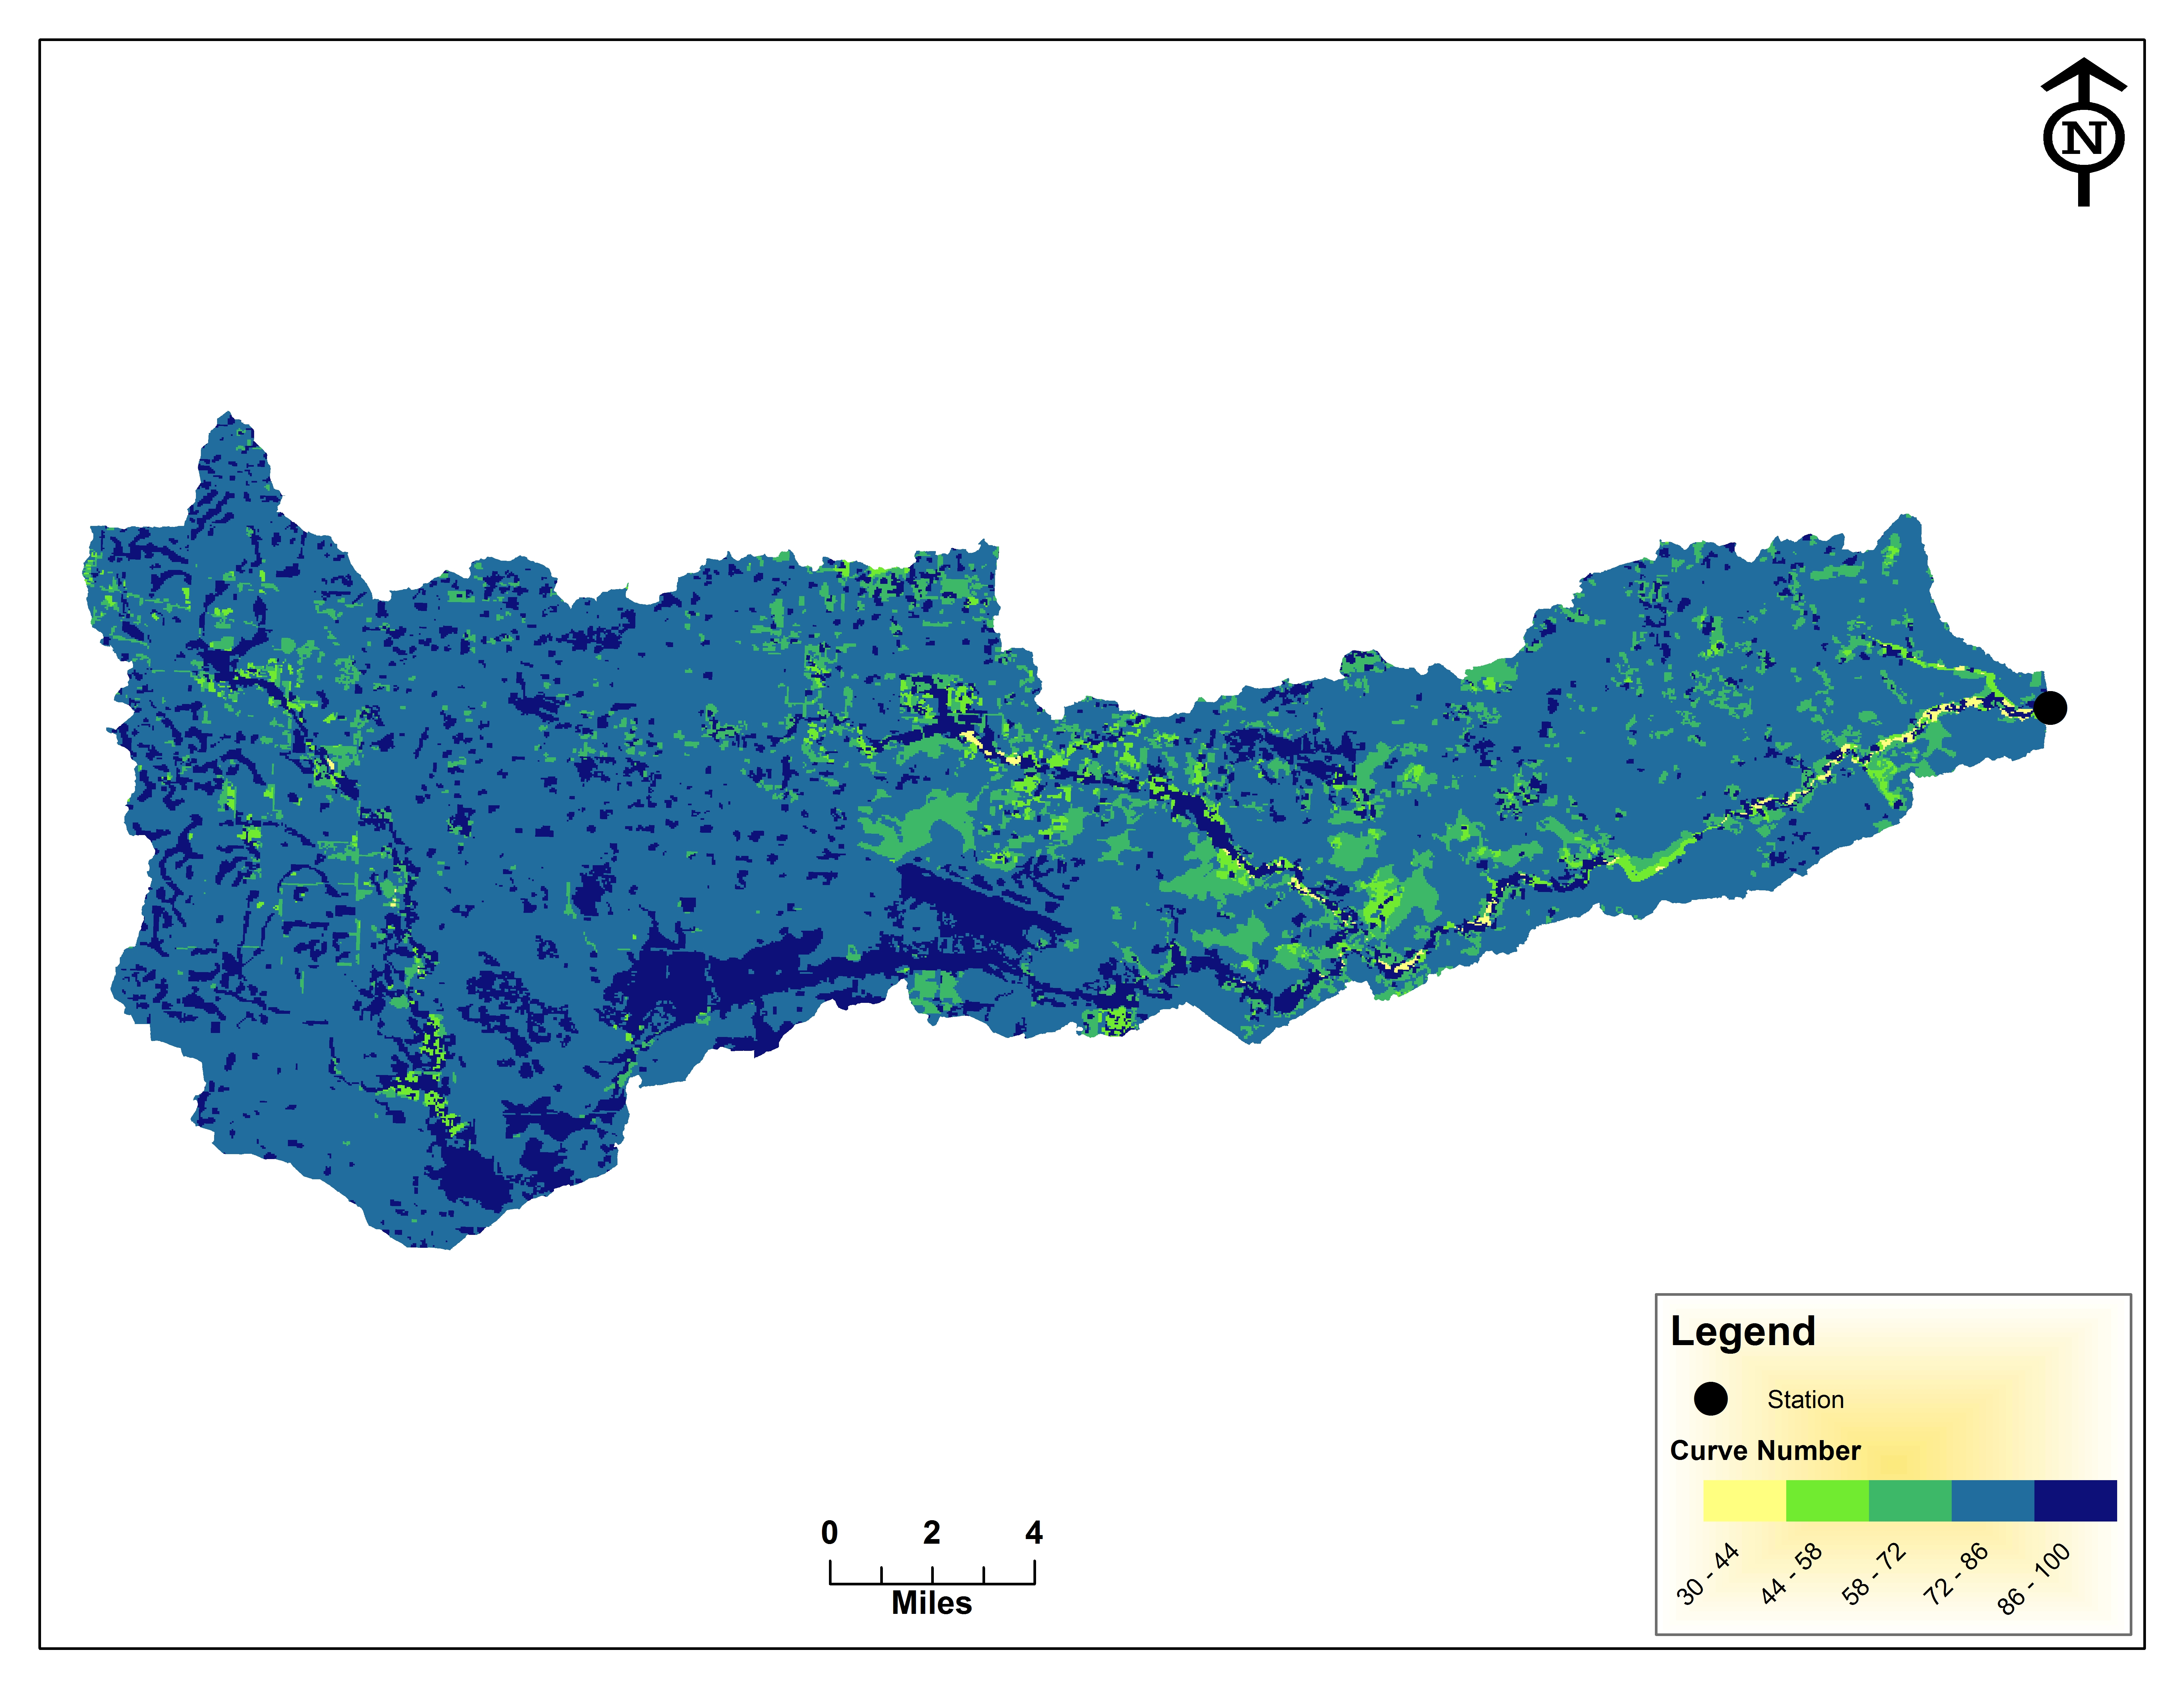
\includegraphics[width=16cm]{CN_2}
		\end{center}
		\caption{Curve Number Map}\label{cn}
	\end{figure}~
	
	~\item \textbf{Calculate the area-weighted curve number for your watershed. (Show your calculations/code).}\\~
	
	The area-weighted curve number can be obtained using Equation 1:\\
	\begin{equation}
	\overline{CN}=\frac{\sum_{i=1}^{n} CN_i \times A_i}{\sum_{i=1}^{n} A_i}
	\end{equation}\\
	Since we used a fishnet to obtain the CN distribution map, the area associated with each cell is same for all and equal to cell size. So the CN calculation can be simplified as follows:\\
	$$\overline{CN}=\frac{A_{cell} \times \sum_{i=1}^{n} CN_i}{A_{cell}\times n} =\frac{\sum_{i=1}^{n} CN_i}{n}$$\\
	
	where n is the total number of cells in fishnet ($279673$ active cells for CN). Calling a query on curve number attribute in fishnet data results in CN summation equals to $23073022$. Then we have:
	
	$$\overline{CN}=\frac{\sum_{i=1}^{n} CN_i}{n}=\frac{23073022}{279673}\approx82$$\\
	
	It should be considered that average curve number of 82 has been obtained with assumptions made regards to reclassification of LULD and SHG data.
	
\end{enumerate}

\newpage

\end{document}